\section{Several modern programming languages}

There is no uniform definition for MPL. Many researchers define it in different ways, such as finding connections between software engineering and the development of MPLs or elaborating around abstractions. The above are correct in their respective fields, and here the definition is abstracted and extended to adapt to more domains. By studying the intersection of different definitions, a more general definition of MPLs derives. It is an obvious fact, that as the practice of programming languages continues to deepen, so does the definition of MPL. This is because PLT is a field where practice and theory go hand in hand. Although its definition is constantly changing, some core elements remain the same. Here are a few features of MPLs.

\begin{enumerate}
    \item Substance over form. It should provide descriptive grammatical structures, rather than hand-in-hand telling the machine what to do. This item emphasizes the abstraction of machine functions.
    \item Semantic Consistency. For similar grammatical structures, there should be similar grammatical functions.
    \item Syntax bootstrapping. For non-core grammatical features, based on following semantic consistency, they should be composed of core grammatical features.
    \item Paradigm fusion. Multiple programming paradigms should be provided without forcing users to use a particular programming paradigm.
\end{enumerate}

\subsection{Select modern programming languages to be analyzed}

For the selection of programming language, the first thing is to pay attention to the most popular trend at the moment, so the selected programming language must cover the most commonly used. Secondly, there are many classification standards for programming languages. For each division standard, the selected programming language should cover most of the options. Then, it should focus on highlighting the new programming language with excellent design in recent years. These programming languages have absorbed the advantages of past programming languages and improved their inherent shortcomings. From these selected MPLs, we can see the development trend of application-oriented programming languages over the years.

According to the data of the *IEEE spectrum*, the top five most popular programming languages in 2021 are Python, Java, C, C ++, and JavaScript. An exception case is C, which provides low-level access to computer systems. To be precise, the syntax design of the C language does not conform to any of the features of MPL. And for the four remaining popular programming languages mentioned above, they are still helpful even though they are not exactly in line with the features of MPL. In the era when these languages were first created, they emerged as representatives of MPLs. Therefore these four past programming languages are compared with the emerging MPLs.

Based on the above-mentioned MPL features, several programming languages were selected and arranged in order of popularity, resulting in Go, Swift, Dart, Rust and Kotlin (where Swift and Dart are equally popular). Coincidentally, these languages are also released in this order sequentially. In addition, all of these languages have similar type systems and all support AOT compilation, and although not all use garbage collection memory management, they all move away from manual memory management. These are all common features of MPLs in today's application environment.

\begin{table*}[ht]
    \caption{selected-languages}
    \label{tab:selected-languages}
    \begin{center}
        \begin{tabular}{ccccccc}
            \toprule
            Language & Programming Paradigm & Type System & Compilation Mode & Memory Model &
            Release Date & Application Scenarios \\
            \midrule
            Python & Multi-paradigm & Dynamically, Strongly & JIT & GC & 1991 & Web,
            Enterprise, Embedded \\
            Java & Multi-paradigm & Statically, Strongly & AOT & GC & 1995 & Web,
            Mobile, Enterprise \\
            C++ & Multi-paradigm & Statically, Weakly & AOT & Manual & 1983 & Mobile,
            Enterprise, Embedded \\
            JavaScript & Multi-paradigm & Untyped & JIT & GC & 1995 &
            Web \\
            Go & Multi-paradigm & Statically, Strongly & AOT & GC & 2009 & Web,
            Enterprise \\
            Swift & Multi-paradigm & Statically, Strongly & AOT & ARC & 2014 &
            Mobile, Enterprise \\
            Dart & Multi-paradigm & Statically, Strongly & AOT\&JIT & GC & 2011 &
            Web, Mobile \\
            Rust & Multi-paradigm & Statically, Strongly & AOT & Ownership & 2015 &
            Web, Enterprise, Embedded \\
            Kotlin & Multi-paradigm & Statically, Strongly & AOT\&JIT & GC & 2016 &
            Web, Mobile \\
            \bottomrule
        \end{tabular}
    \end{center}
\end{table*}

\subsection{Evolution of modern programming languages}

\begin{figure}[htbp]
    \centerline{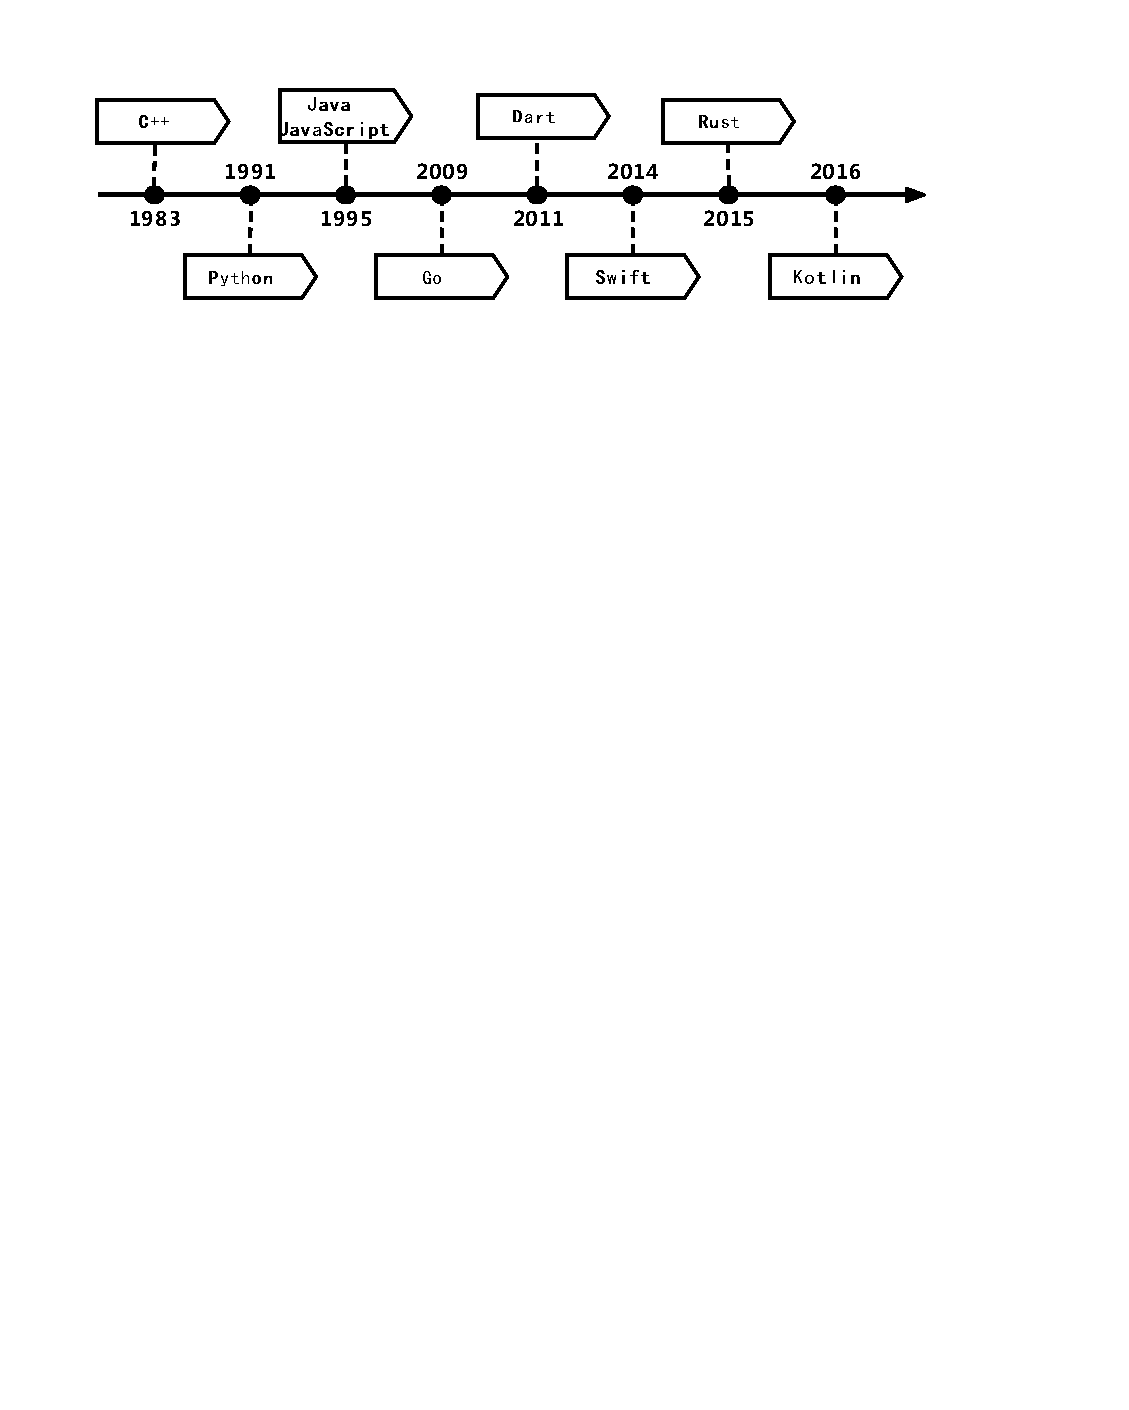
\includegraphics[scale=0.6]{figures/timeline}}
    \caption{timeline}
    \label{fig:timeline}
\end{figure}

Programming languages have a considerable degree of time sensitivity. For different programming languages from different eras spanning a large period of time, one of them is still more "outdated" than the other, although they all conform to the above features of modern programming languages. This is due to the fact that the above principles are in conflict in the time dimension. Indeed, substance over form requires programming languages to abstract the syntactic features required by specific application scenarios, but the needs of application scenarios change over time as they are upgraded through technological iterations. At this point, if you want to add new syntactic features to the original programming language, it is easy to destroy the principle of syntactic bootstrapping and semantic consistency. Therefore, a better solution at this point is to design a new programming language to meet the new requirements from the language design level.

However, there are also factors that hinder the progress of programming language obsolescence. Programming languages take a long time to go from prototype to mass adoption, and during this time, programming languages gradually improve their ecosystem. The ecosystem is like a dense web, and it is almost impossible to phase out programming languages completely once they start to be used on a large scale. For developing computer applications, the ideal state would be for new programming languages to be compatible with older programming languages, thus allowing the new programming languages to inherit the old ecosystem, a typical example being C and C++. However, due to some force majeure, the new programming language is not compatible with the old one. In this case, the compatibility of the programming language ecosystem can be achieved through virtual machines, but only if both the new one and the old one are based on the same virtual machine, a typical example being Java and Kotlin. In addition, there is a more general approach where the new programming language implements the data interface of the old programming language. This is how most languages interact with C/C++. However, there are greater functional limitations to doing so. In the development of programming languages, each one is compatible with some of the past.

The trend is still to phase out old programming languages, but in a slower manner. While the ecosystem of the past can be reused through compatibility with older programming languages, the maintenance challenges caused by older programming languages remain insurmountable. Therefore, compatibility with older programming languages is a compromise. First, develop the new programming language itself through the old ecosystem. Second, restructure the old ecosystem with the new programming language. Eventually, achieve a mass phase-out of the old programming languages.